\documentclass[a4paper,14pt]{article}

%%% Работа с русским языком
\usepackage{cmap}					% поиск в PDF
\usepackage{mathtext} 				% русские буквы в формулах
\usepackage[T2A]{fontenc}			% кодировка
\usepackage[utf8]{inputenc}			% кодировка исходного текста
\usepackage[english,russian]{babel}	% локализация и переносы
\usepackage{indentfirst}
\frenchspacing

\newcommand{\vyp}{\ensuremath{\hookrightarrow}}
\renewcommand{\epsilon}{\ensuremath{\varepsilon}}
\renewcommand{\phi}{\ensuremath{\varphi}}
\renewcommand{\kappa}{\ensuremath{\varkappa}}
\renewcommand{\le}{\ensuremath{\leqslant}}
\renewcommand{\leq}{\ensuremath{\leqslant}}
\renewcommand{\ge}{\ensuremath{\geqslant}}
\renewcommand{\geq}{\ensuremath{\geqslant}}
\renewcommand{\emptyset}{\varnothing}
\newcommand{\Ra}{\ensuremath{\Rightarrow}}
\newcommand{\ra}{\ensuremath{\rightarrow}}
\newcommand{\LRa}{\ensuremath{\Leftrightarrow}}
\newcommand{\tbf}{\textbf}
\newcommand{\ov}{\ensuremath{\overline}}
\newcommand{\CC}{\ensuremath{\mathbb{C}}}
\newcommand{\RR}{\ensuremath{\mathbb{R}}}
\newcommand{\NN}{\ensuremath{\mathbb{N}}}
\newcommand{\QQ}{\ensuremath{\mathbb{Q}}}
\newcommand{\ZZ}{\ensuremath{\mathbb{Z}}}

%%% Дополнительная работа с математикой
\usepackage{amsmath,amsfonts,amssymb,amsthm,mathtools} % AMS
\usepackage{icomma} % "Умная" запятая: $0,2$ --- число, $0, 2$ --- перечисление

%% Номера формул
%\mathtoolsset{showonlyrefs=true} % Показывать номера только у тех формул, на которые есть \eqref{} в тексте.
%\usepackage{leqno} % Нумереация формул слева

%% Свои команды
\DeclareMathOperator{\sgn}{\mathop{sgn}}

%% Перенос знаков в формулах (по Львовскому)
\newcommand*{\hm}[1]{#1\nobreak\discretionary{}
{\hbox{$\mathsurround=0pt #1$}}{}}



%%% Работа с картинками
\usepackage{graphicx}  % Для вставки рисунков
\graphicspath{{images/}{images2/}}  % папки с картинками
\setlength\fboxsep{3pt} % Отступ рамки \fbox{} от рисунка
\setlength\fboxrule{1pt} % Толщина линий рамки \fbox{}
\usepackage{wrapfig} % Обтекание рисунков текстом

%%% Работа с таблицами
\usepackage{array,tabularx,tabulary,booktabs} % Дополнительная работа с таблицами
\usepackage{longtable}  % Длинные таблицы
\usepackage{multirow} % Слияние строк в таблице

%%% Теоремы
\theoremstyle{plain} % Это стиль по умолчанию, его можно не переопределять.
\newtheorem{theorem}{Теорема}[section]
\newtheorem{proposition}[theorem]{Утверждение}
 
\theoremstyle{definition} % "Определение"
\newtheorem{corollary}{Следствие}[theorem]
\newtheorem{problem}{Задача}[section]
 
\theoremstyle{remark} % "Примечание"
\newtheorem*{nonum}{Решение}

%%% Программирование
\usepackage{etoolbox} % логические операторы

%%% Страница
\usepackage{extsizes} % Возможность сделать 14-й шрифт
\usepackage{geometry} % Простой способ задавать поля
	\geometry{top=20mm}
	\geometry{bottom=20mm}
	\geometry{left=5mm}
	\geometry{right=15mm}
 %
\usepackage{fancyhdr} % Колонтитулы
 	\pagestyle{fancy}
 	\renewcommand{\headrulewidth}{1pt}  % Толщина линейки, отчеркивающей верхний колонтитул
%\fancypagestyle{firstpage}{
	\rhead{\large{Исыпов Илья}}
%}
% 	\lfoot{Нижний левый}
% 	\rfoot{\large{Рябых Владислав, Б05-905}}
% 	\rhead{Верхний правый]}
% 	\chead{Верхний в центре}
 	\lhead{\large{Рябых Владислав}}
%	\cfoot{Нижний в центре} % По умолчанию здесь номер страницы

\usepackage{setspace} % Интерлиньяж
\onehalfspacing % Интерлиньяж 1.5
%\doublespacing % Интерлиньяж 2
%\singlespacing % Интерлиньяж 1

\usepackage{lastpage} % Узнать, сколько всего страниц в документе.

\usepackage{soul} % Модификаторы начертания

\usepackage{hyperref}
\usepackage[usenames,dvipsnames,svgnames,table,rgb]{xcolor}
\hypersetup{				% Гиперссылки
    unicode=true,           % русские буквы в раздела PDF
    pdftitle={Заголовок},   % Заголовок
    pdfauthor={Автор},      % Автор
    pdfsubject={Тема},      % Тема
    pdfcreator={Создатель}, % Создатель
    pdfproducer={Производитель}, % Производитель
    pdfkeywords={keyword1} {key2} {key3}, % Ключевые слова
    colorlinks=true,       	% false: ссылки в рамках; true: цветные ссылки
    linkcolor=red,          % внутренние ссылки
    citecolor=black,        % на библиографию
    filecolor=magenta,      % на файлы
    urlcolor=cyan           % на URL
}

\usepackage{csquotes} % Еще инструменты для ссылок

%\usepackage[style=authoryear,maxcitenames=2,backend=biber,sorting=nty]{biblatex}

\usepackage{multicol} % Несколько колонок

\usepackage{tikz} % Работа с графикой
\usepackage{pgfplots}
\usepackage{pgfplotstable}

\usepackage{caption}
\long\def\comment{}
\setlength{\abovecaptionskip}{7pt}
\setlength{\belowcaptionskip}{7pt}


\begin{document}
\author{Рябых Владислав и Исыпов Илья, Б05-905}
\title{\tbf{3.5.3. Релаксационные колебания}}
\maketitle

\tbf{Цель работы:} изучение вольт-амперной характеристики нормального
тлеющего разряда; исследование релаксационного генератора на
стабилитроне.

\tbf{В работе используются:} стабилитрон СГ-2 (газонаполненный диод) на монтажной панели, амперметр, магазин сопротивлений, магазин ёмкостей, источник
питания, осциллограф (ЭО), генератор звуковой частоты (ЗГ).


\section*{Теория}
Колебательные системы, как правило имеют два накопителя энергии, между которыми происходит ее перекачка. В контуре, содержащем конденсатор и катушку индуктивности, электрическая энергия переходит в магнитную и обратно.

Встречаются, однако, колебательные системы, содержащие всего один накопитель энергии. Рассмотрим в качестве примера электрическую цепь, содержащую конденсатор и сопротивление без самоиндукции. Разряд конденсатора через сопротивление представляет собой апериодический процесс. Разряду, однако, можно придать периодический характер, возобновляя заряд конденсатора через постоянные промежутки времени. Колебания в этом случае являются совокупностью двух апериодических процессов -- процесса зарядки конденсатора и процесса его разрядки. Такие колебания называются релаксационными. 



\begin{figure}[!h]
	\parbox[!h]{0.5\textwidth}{\null
		\centering
		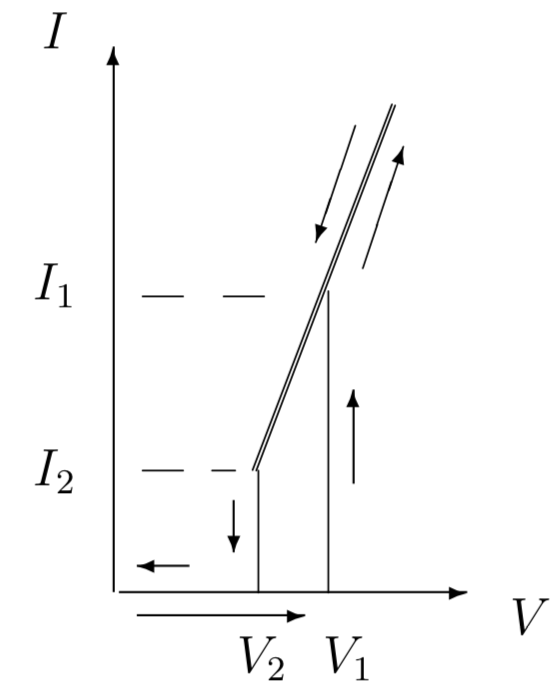
\includegraphics[width = 5cm]{1} \\
		Рис. 1 -- ВАХ стабилитрона с последовательно включенным резистором}
	\parbox[!h]{0.5\textwidth}{\null
		\centering
		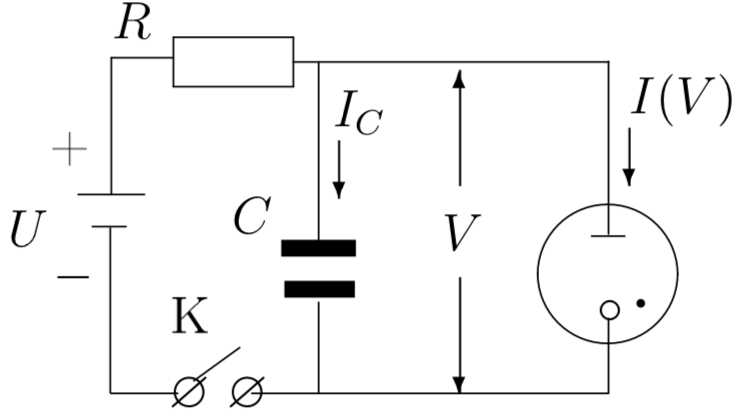
\includegraphics[width = 8.5cm]{2} \\
		Рис. 2 -- Принципиальная схема релаксационного генератора}
\end{figure}

В нашей установке роль "ключа", обеспечивающего попеременную зарядку и разрядку конденсатора играет газоразрядный диод. Зависимость тока от напряжения для газоразрядной лампы не подчиняется закону Ома и характеризуется рядом особенностей (рис. 1). При малых напряжениях лампа не пропускает тока, ток в лампе возникает только в том случае, если разность потенциалов на ее электродах достигает напряжения зажигания $V_1$. При этом скачком устанавливается конечная сила тока $I_1$ -- в лампе возникает нормальный тлеющий разряд. При дальнейшем незначительном увеличении напряжения сила тока заметно возрастает по закону, близкому к линейному. Нормальный тлеющий разряд -- стабилизатор напряжения, отсюда второе название лампы -- стабиловольт. 

Если начать уменьшать напряжение на горящей лампе, то при напряжении равном $V_1$ лампа еще не гаснет, и сила тока продолжает уменьшаться. Лампа перестает пропускать ток лишь при напряжении гашения $V_2$, которое обычно существенно меньше $V_1$. Сила тока при этом скачком падает от значения $I_2$ до нуля.

Рассмотрим схему релаксационного генератора, изображенную на рис. 2. Пусть напряжение батареи $U$ больше напряжения зажигания $V_1$. В обозначениях, принятых на схеме, справедливо уравнение $$I_C + I(V) = \dfrac{U-V}{R}$$ или 

\begin{equation}
C\dfrac{dV}{dt} + I(V) = \dfrac{U-V}{R}.
\label{eq1}
\end{equation}

В стационарном режиме работы, когда напряжение $V$ на конденсаторе постоянно и $dV/dt = 0$, ток через лампу равен 

\begin{equation}
I_{\text{ст}} = \dfrac{U-V}{R}.
\label{eq2}
\end{equation}

При $V = V_2$ получаем выражение для критического сопротивления:

\begin{equation}
R_{\text{кр}} = \dfrac{U-V_2}{I_2}.
\label{eq3}
\end{equation}

\begin{figure}[!h]
	\centering
	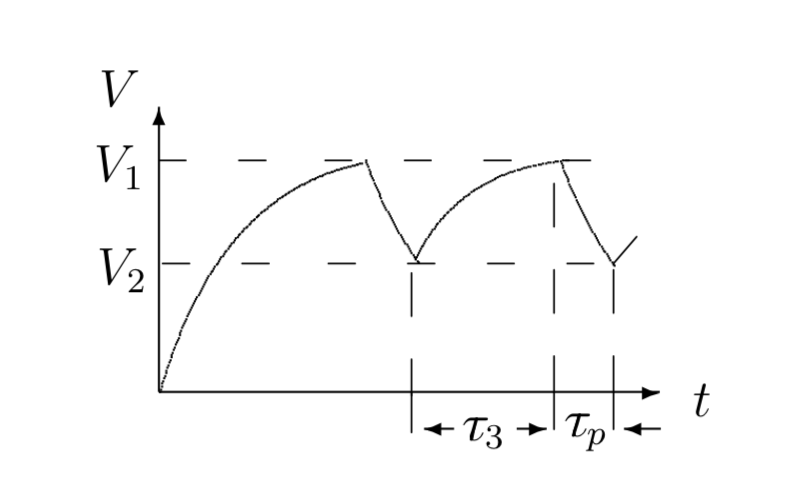
\includegraphics[width = 7cm]{3} \\
	Рис. 3 -- Осциллограмма релаксационных колебаний
\end{figure}

Рассмотрим, как происходит колебательный процесс. Пусть в начале опыта ключ разомкнут. Замкнем ключ, конденсатор $C$ начинает заряжаться через сопротивление $R$, напряжение на нем начинает увеличиваться (рис. 3). Как только оно достигнет напряжения зажигания лампы $V_1$, лампа начинает проводить ток, причем прохождение тока сопровождается разрядкой конденсатора. В самом деле, батарея $U$, подключенная через большое сопротивление $R$, не может поддерживать необходимую для горения лампы величину тока. Во время горения лампы конденсатор разряжается, и когда напряжение на нем достигает потенциала гашения, лампа перестает проводить ток, а конденсатор вновь начнет заряжаться. Возникают релаксационные колебания с амплитудой, равной $(V_1-V_2)$.

Рассчитаем период колебаний. Полное время одного периода колебаний $T$ состоит из суммы времени зарядки $\tau_{\text{з}}$ и времени разрядки $\tau_{\text{р}}$, но если сопротивление $R$ существенно превосходит сопротивление зажженой лампы, то получаем, что $\tau_{\text{з}} \gg \tau_{\text{р}}$ и $T \approx \tau_{\text{з}}$ (этим случаем мы и ограничимся).

Во время зарядки конденсатора лампа не горит ($I(V)=0$), и уравнение \eqref{eq1} принимает вид 

\begin{equation}
RC \dfrac{dV}{dt} = U-V.
\label{eq4}
\end{equation}

Будем отсчитывать время с момента гашения лампы, так что $V=V_2$ при $t=0$ (рис. 3). Решив уравнение \eqref{eq4}, найдем 

\begin{equation}
V = U - (U-V_2)e^{-t/RC}.
\label{eq5}
\end{equation}

В момент зажигания $t = \tau_{\text{з}}, V = V_1$, поэтому

\begin{equation}
V_1 = U - (U-V_2)e^{-\tau_{\text{з}}/RC}.
\label{eq6}
\end{equation}

Из уравнений \eqref{eq5} и \eqref{eq6} нетрудно выразить период колебаний:

\begin{equation}
T \approx \tau_{\text{з}} = RC \ln \dfrac{U-V_2}{U-V_1}.
\label{eqT}
\end{equation}

\section*{Ход работы}
\subsection*{Характеристика стабилитрона}

Соберем схему представленную на рис. 4. Снимем ВАХ стабилитрона, данные занесем в таблицу \ref{tab1} ($r = 5.4$ кОм). 

	\begin{table}[bhtp]
		\begin{center}
		\begin{tabular}{|c|c|}
			\hline
			$U$, В & $I$, мA \\ \hline
			0.0    & 0.00    \\ \hline
			10.0   & 0.00    \\ \hline
			15.0   & 0.00    \\ \hline
			65.0   & 0.00    \\ \hline
			75.0   & 0.00    \\ \hline
			85.0   & 0.00    \\ \hline
			89.4   & 3.17    \\ \hline
			99.3   & 5.04    \\ \hline
			104.3  & 6.01    \\ \hline
			110.0  & 6.98    \\ \hline
			115.0  & 7.85    \\ \hline
			119.1  & 8.64    \\ \hline
			125.5  & 9.74    \\ \hline
			129.5  & 10.40   \\ \hline
			134.5  & 11.31   \\ \hline
			140.0  & 12.33   \\ \hline
			145.6  & 13.33   \\ \hline
			152.3  & 14.51   \\ \hline
			158.7  & 15.63   \\ \hline
			150.9  & 14.29   \\ \hline
			147.1  & 13.62   \\ \hline
			141.7  & 12.66   \\ \hline
			136.7  & 11.84   \\ \hline
			126.7  & 10.00   \\ \hline
			121.5  & 9.06    \\ \hline
			116.1  & 8.15    \\ \hline
			110.3  & 7.10    \\ \hline
			105.7  & 6.28    \\ \hline
			101.0  & 5.45    \\ \hline
			96.0   & 4.57    \\ \hline
			91.1   & 3.67    \\ \hline
			86.2   & 2.78    \\ \hline
			80.3   & 1.38    \\ \hline
			78.8   & 0.00    \\ \hline
		\end{tabular}
		\caption{ВАХ стабилитрона}\label{tab1}
		\end{center}
	\end{table}

Получаем значения: $$V_1 = 89.4 \text{ В},  \ \ V_2 = 80.3 \text{ В}, $$ $$I_1 = 3.17 \text{ мА}, \ \  I_2 = 1.38 \text{ мА}.$$

\begin{figure}[!h]
	\centering
	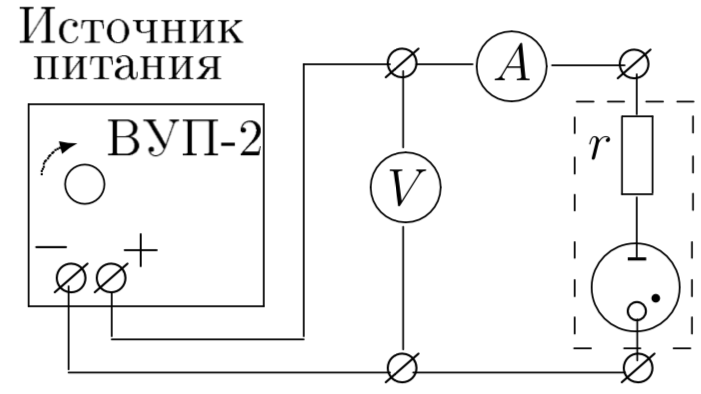
\includegraphics[width = 8cm]{4} \\
	Рис. 4 -- Схема установки для изучения характеристик стабилитрона
\end{figure}

Построим графики зависимостей $I= f(V)$ для системы, состоящей из стабилитрона и дополнительного сопротивления по данным таблицы \ref{tab1}, а также для стабилитрона без дополнительного сопротивления (вычитая падение напряжения на сопротивлении $r$ при каждом токе), см. рис. 5 -- 6. По графикам видно, что относительное изменение тока и напряжения на стабилитроне больше на первом графике.

\begin{center}
\begin{figure}[bhtp]
	\centering
	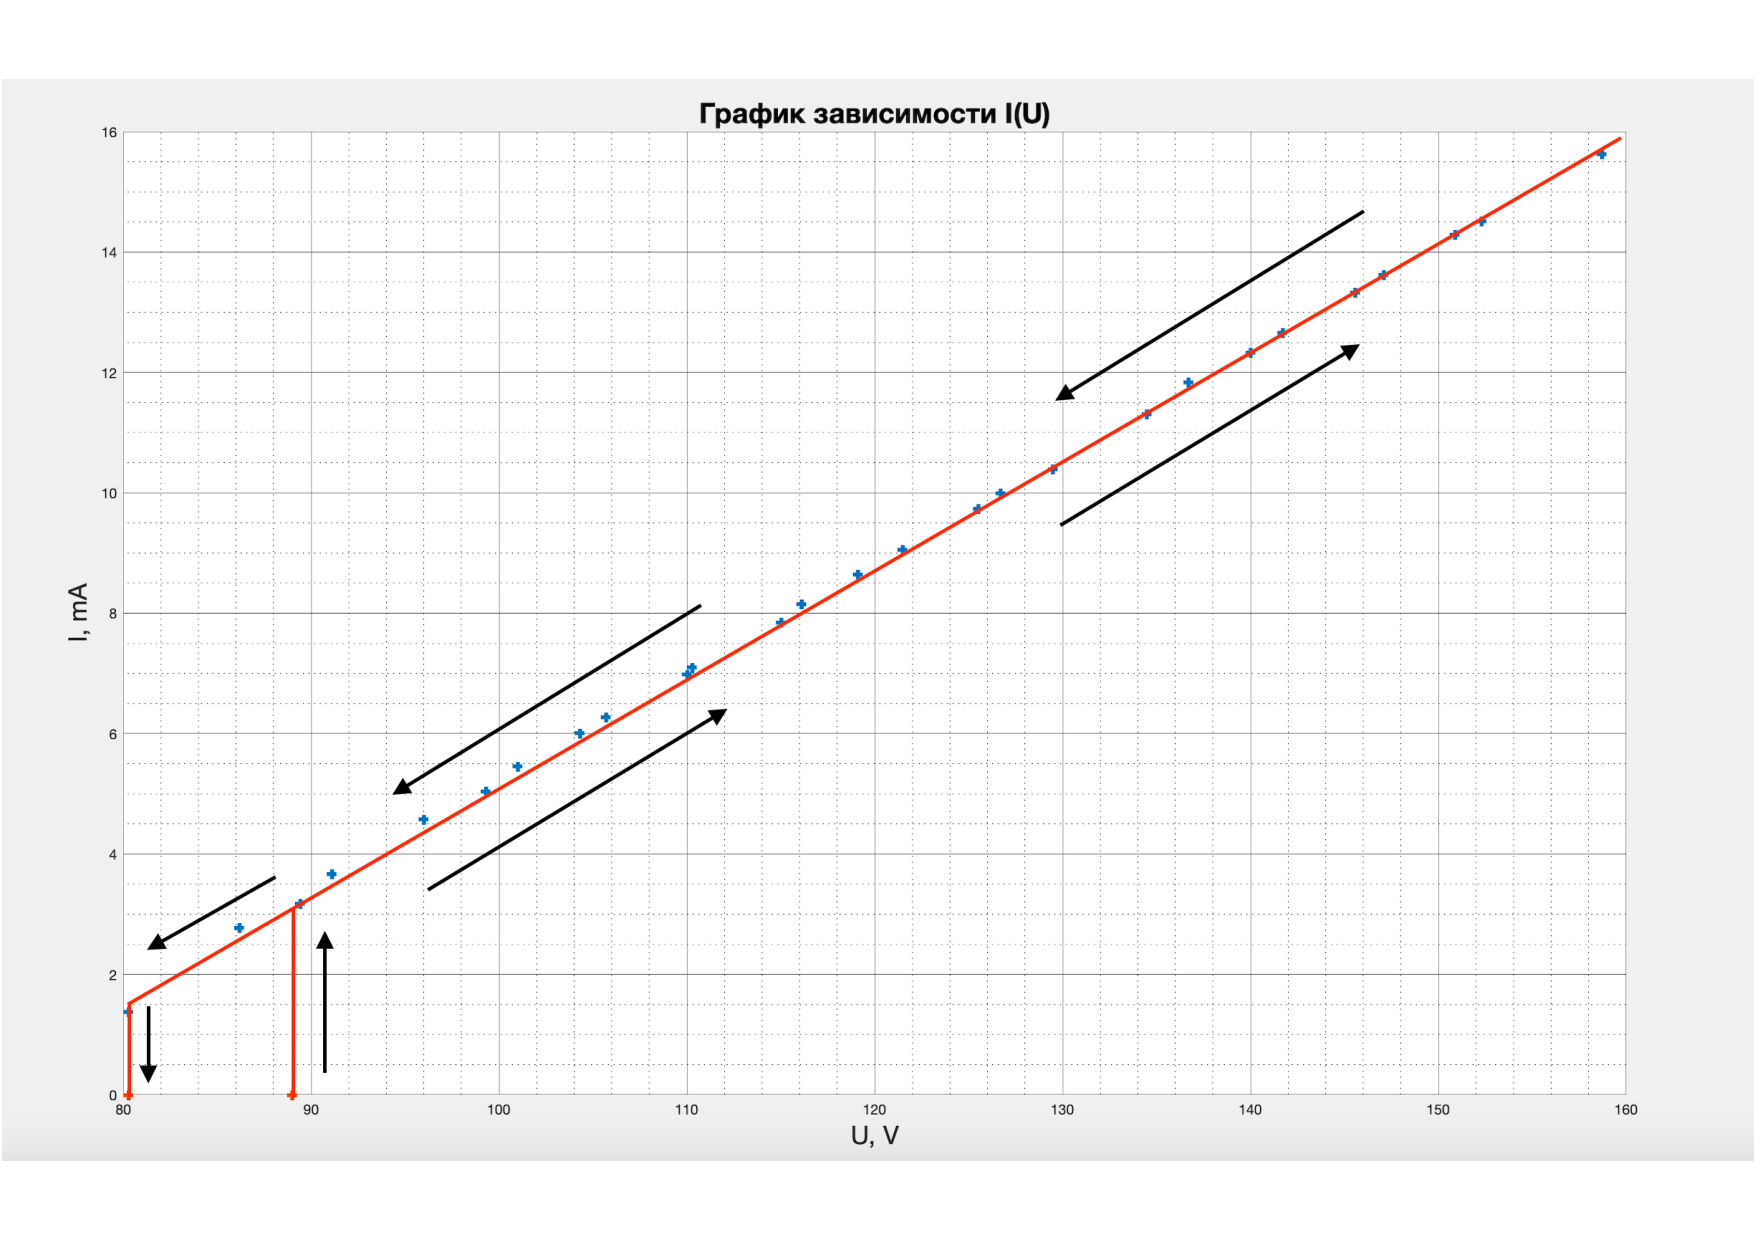
\includegraphics[width=0.85\linewidth]{gg1.pdf} \\
	Рис. 5 -- Графики зависимостей $I = f(V)$ для стабилитрона с $r$
\end{figure}
\end{center}

\begin{center}
	\begin{figure}[bhtp]
		\centering
		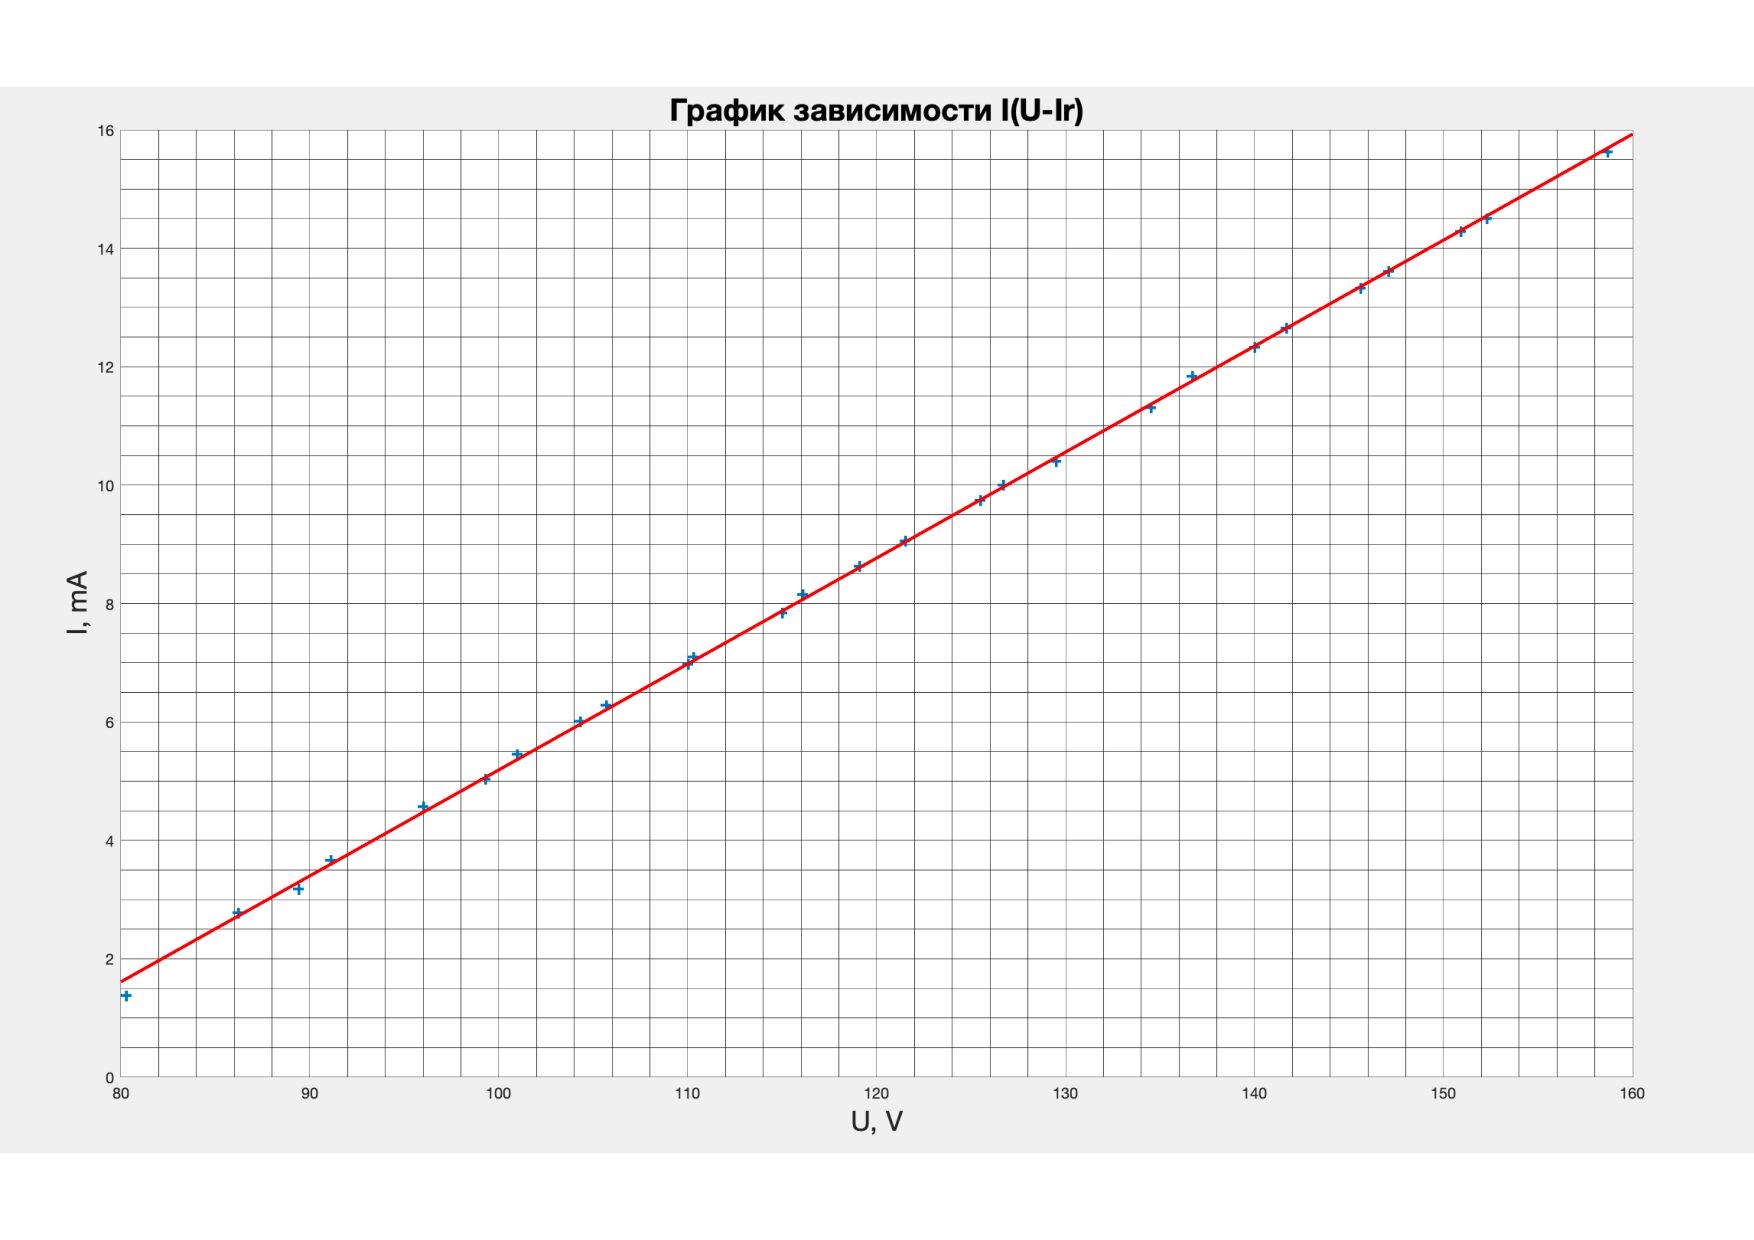
\includegraphics[width=0.85\linewidth]{gg2.pdf} \\
		Рис. 6 -- Графики зависимостей $I= f(V)$ для стабилитрона без $r$
	\end{figure}
\end{center}


\subsection*{Осциллограммы релаксационных колебаний}

\begin{figure}[bhtp]
	\centering
	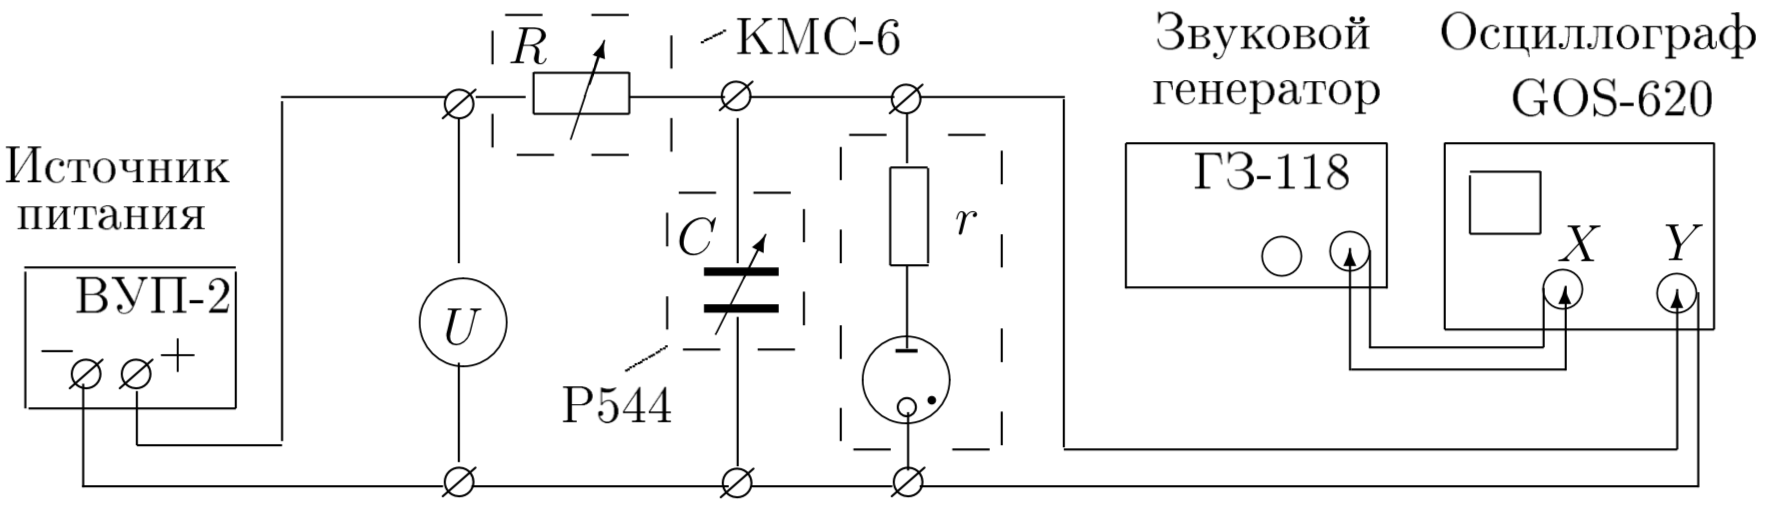
\includegraphics[width =14cm]{5} \\
	Рис. 7 -- Схема экспериментальной установки для исследования релаксационных колебаний
\end{figure}

Соберем схему, согласно рис. 7. По полученным пилообразным картинам оценим соотношение между временем зарядки разрядки конденсатора: 
$$\dfrac{\tau_{\text{з}}}{\tau_{\text{р}}} \approx \dfrac{47}{3},$$
следовательно можно считать, что время разрядки сильно меньше времени зарядки.

Теоретическое критическое сопротивление определяется по формуле \eqref{eq3} равно $R_{\text{кр}} = 81.4$ кОм, экспериментальное значение, при котором исчезают
колебания $R_{\text{эксп}} = 100$ кОм.

Также мы убедились в том, что колебания пропадают при увеличении напряжения при постоянном сопротивление, если это сопротивление не сильно превышает критическое.

\subsection*{Фигуры Лиссажу и частота колебаний}

Занесем опытные данные зависимости частоты колебаний $\nu$  от емкости $C$, а также при постоянной емкости, но при разных сопротивлениях от максимально до критического в таблицы \ref{tab2}, \ref{tab3}. Соответствующие им теоретические данные, рассчитаны по формуле \eqref{eqT}.

\begin{table}[bhtp]
\begin{center}
\begin{tabular}{|c|c|c|}
	\hline
	$\nu$, Гц & $C$, мкФ & $T$, мc \\ \hline
	14        & 0.040    & 71.43 \\ \hline
	18        & 0.030    & 55.56 \\ \hline
	26        & 0.020    & 38.46 \\ \hline
	57        & 0.010    & 17.54 \\ \hline
	65        & 0.009    & 15.38 \\ \hline
	89        & 0.007    & 11.24 \\ \hline
\end{tabular}
\caption{Результаты измерений}\label{tab2}
\end{center}
\end{table}

\begin{table}[bhtp]
	\begin{center}
		\begin{tabular}{|c|c|c|}
			\hline
			$R$, кОм & $\nu$, Гц & $T$, мс \\ \hline
			400      & 20        & 50.00   \\ \hline
			350      & 33        & 30.30   \\ \hline
			300      & 37        & 27.03   \\ \hline
			250      & 45        & 22.22   \\ \hline
			200      & 56        & 17.86   \\ \hline
			150      & 79        & 12.66   \\ \hline
			100      & 120       & 8.33    \\ \hline
		\end{tabular}
		\caption{Результаты измерений}\label{tab3}
	\end{center}
\end{table}

По данным таблиц построим графики зависимостей $T_{\text{эксп}} = f(C)$ и $T_{\text{теор}} = f(C)$ на рис. 8. Аналогичные графики зависимостей построим на рис. 9 для сопротивления $T_{\text{эксп}} = f(R)$ и $T_{\text{эксп}} = f(R)$.

\begin{center}
	\begin{figure}[bhtp]
		\centering
		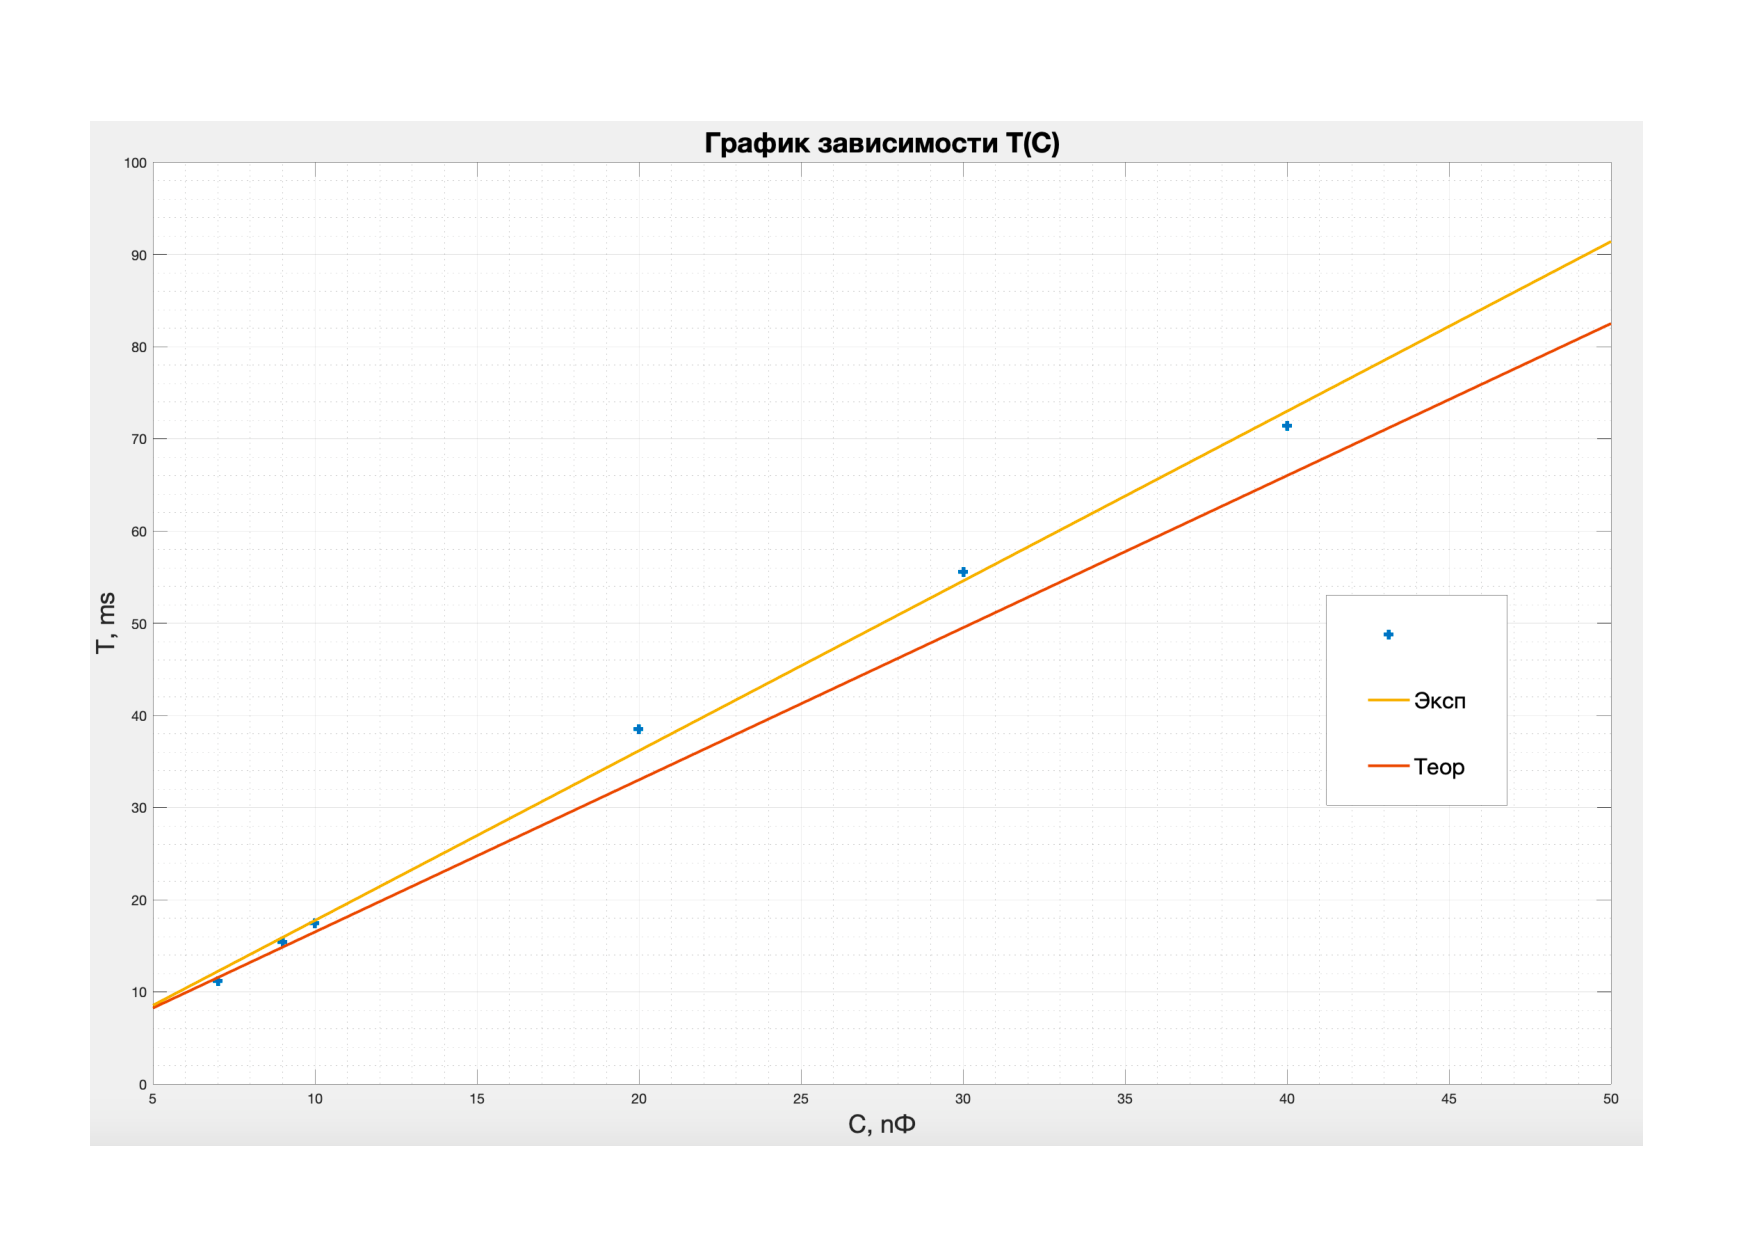
\includegraphics[width=0.85\linewidth]{gg3.pdf} \\
		Рис. 8 -- Графики зависимостей $T_{\text{эксп}} = f(C)$ и $T_{\text{теор}} = f(C)$
	\end{figure}
\end{center}

\begin{center}
\begin{figure}[bhtp]
	\centering
	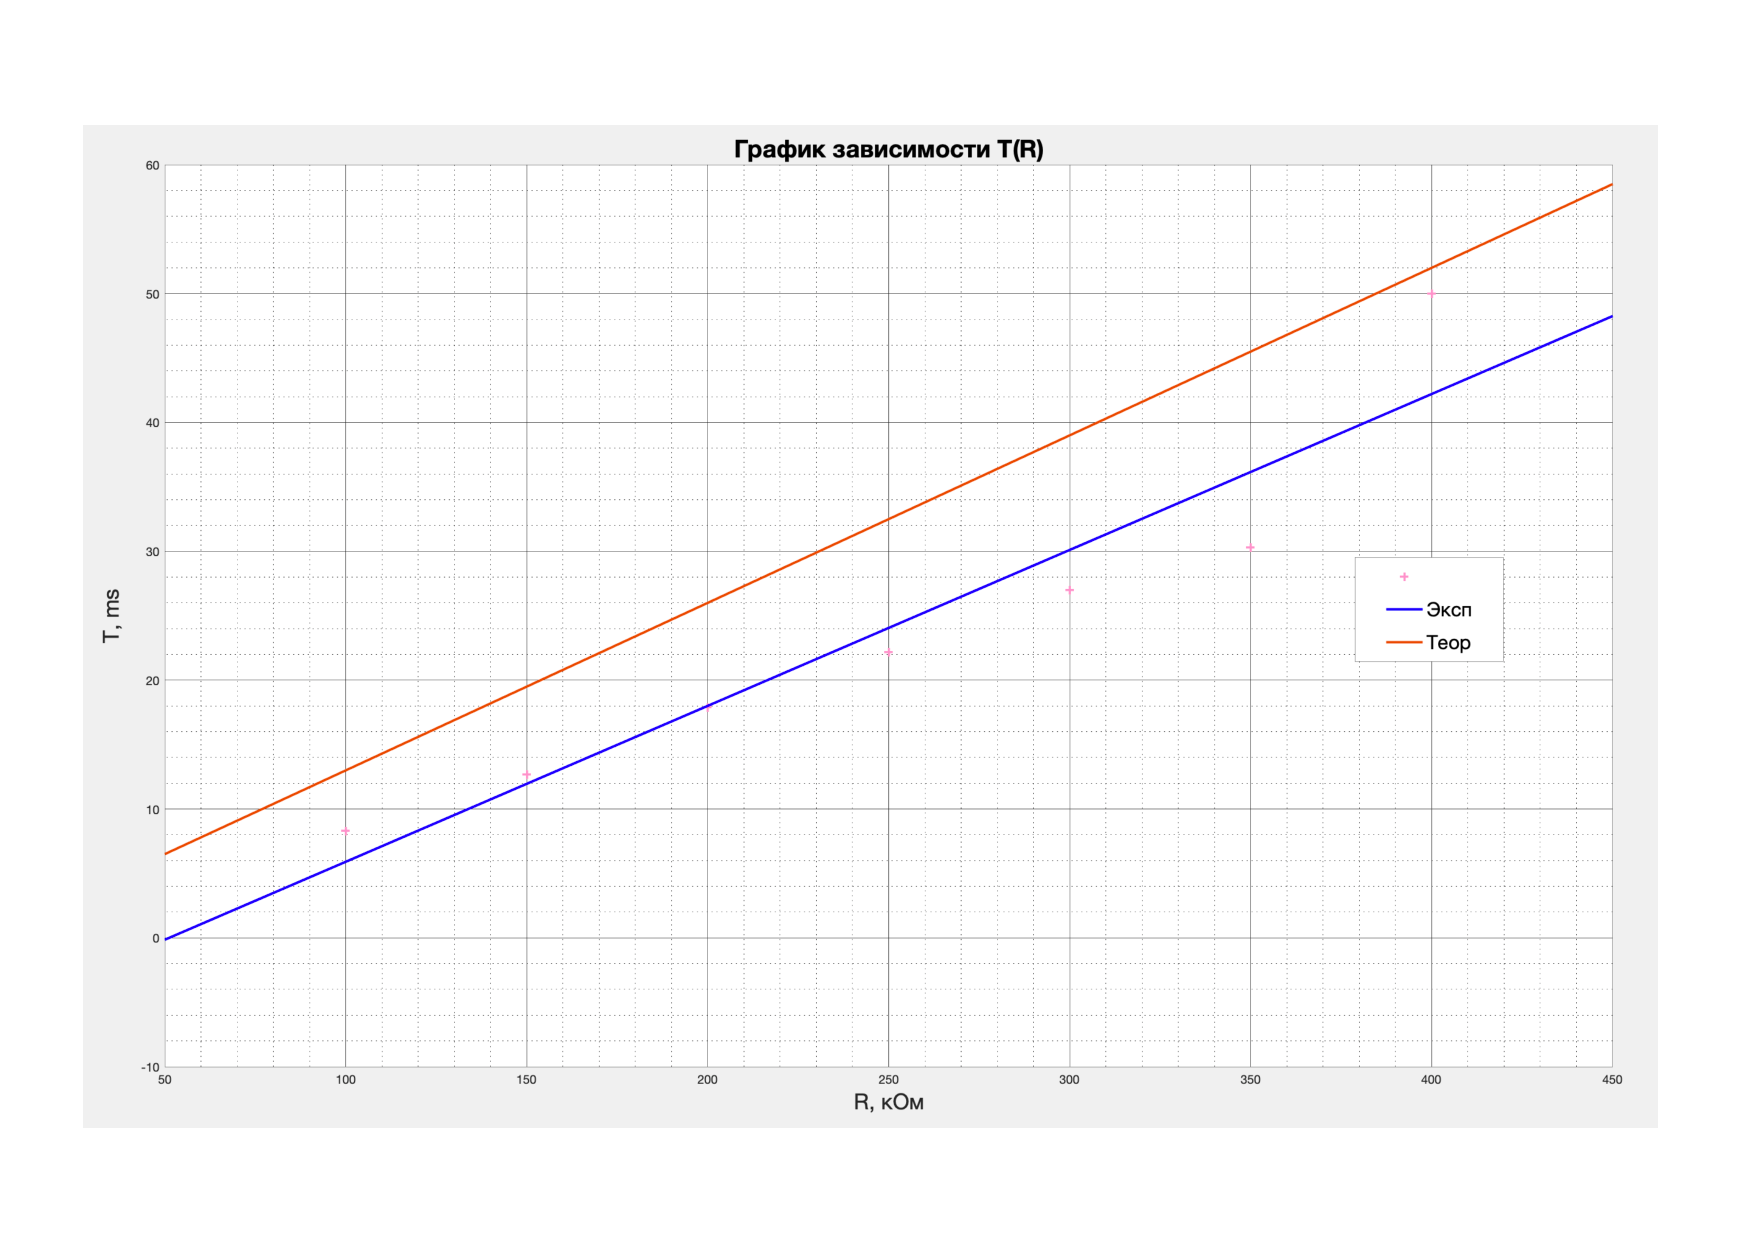
\includegraphics[width=\linewidth]{gg4.pdf} \\
	Рис. 9 -- Графики зависимостей $T_{\text{эксп}} = f(R)$ и $T_{\text{теор}} = f(R)$
\end{figure}
\end{center}

\section*{Выводы}
	В ходе лабораторной работы были рассмотрены процессы установления релаксационных колебаний внутри неоновой газоразрядной лампы. Необходимо отметить, что  наклоны графиков получились совпадающими в пределах погрешности с теоретическими, поэтому можно считать данную теоретическую модель достаточно точной.


\end{document}